%% WARDEN -- IEEE Internet of Things Journal submission
%% Uses the official IEEEtran class when it is installed (Overleaf, TeX Live full).
%% Otherwise falls back to an IEEEtran-equivalent two-column layout (same paper size,
%% text block, column gap, 10-pt Times) so that the page count can be checked offline.
\IfFileExists{IEEEtran.cls}{%
  \documentclass[journal]{IEEEtran}\def\WARDENieee{1}%
}{%
  \documentclass[10pt,twocolumn,letterpaper]{article}%
}
\usepackage[T1]{fontenc}
\usepackage{amsmath,amssymb}
\ifdefined\WARDENieee\else
  \usepackage{mathptmx}
  \usepackage[letterpaper,textwidth=43pc,textheight=58pc,columnsep=1pc,top=54pt,hmargin=0.6625in]{geometry}
  %% IEEEtran-equivalent styling used ONLY when IEEEtran.cls is not installed.
%% On Overleaf / full TeX Live the real IEEEtran class is used and this file is ignored.
\usepackage{titlesec}
\usepackage{caption}
\usepackage{enumitem}
\setlength{\parindent}{1em}
\renewcommand{\baselinestretch}{1.0}
\makeatletter
\renewcommand\normalsize{\@setfontsize\normalsize{10}{12}%
  \abovedisplayskip 5pt plus 2pt minus 2pt\belowdisplayskip\abovedisplayskip
  \abovedisplayshortskip 3pt plus 1pt\belowdisplayshortskip\abovedisplayshortskip}
\normalsize
\renewcommand\footnotesize{\@setfontsize\footnotesize{8}{9}}
\renewcommand\scriptsize{\@setfontsize\scriptsize{7}{8}}
% title block
\def\@maketitle{\newpage\null\vskip -6pt
  \begin{center}{\fontsize{24}{26}\selectfont \@title\par}\vskip 10pt
  {\fontsize{11}{13}\selectfont \@author\par}\end{center}\par\vskip 12pt}
\makeatother
% sections: I. INTRODUCTION / A. Subsection
\renewcommand\thesection{\Roman{section}}
\renewcommand\thesubsection{\thesection-\Alph{subsection}}
\titleformat{\section}{\centering\normalsize\scshape}{\thesection.}{0.5em}{}
\titlespacing*{\section}{0pt}{8pt plus 2pt}{4pt}
\titleformat{\subsection}{\normalsize\itshape}{\Alph{subsection}.}{0.5em}{}
\titlespacing*{\subsection}{0pt}{6pt plus 1pt}{3pt}
% abstract and keywords
\renewenvironment{abstract}{\noindent\small\bfseries\emph{Abstract}---}{\par\vskip 4pt}
\newenvironment{IEEEkeywords}{\noindent\small\bfseries\emph{Index Terms}---}{\par\vskip 6pt}
\usepackage{lettrine}
\newcommand{\IEEEPARstart}[2]{\lettrine[lines=2,findent=1pt,nindent=0pt]{#1}{\MakeUppercase{#2}}}
% captions
\captionsetup[figure]{font=footnotesize,labelsep=period,name=Fig.,skip=3pt}
\captionsetup[table]{font=footnotesize,labelsep=newline,textfont=sc,justification=centering,skip=3pt}
\renewcommand\thetable{\Roman{table}}
\setlist[enumerate]{leftmargin=*,itemsep=1pt,topsep=2pt}
\setlength{\textfloatsep}{8pt plus 2pt minus 2pt}
\setlength{\floatsep}{6pt plus 2pt}
\setlength{\dbltextfloatsep}{8pt plus 2pt minus 2pt}
\setlength{\abovecaptionskip}{3pt}
\newcommand{\IEEEmembership}[1]{\textit{#1}}
\makeatletter\def\@fnsymbol#1{}\makeatother % IEEE: first-page affiliation footnotes are unmarked

\fi
\usepackage{graphicx}
\usepackage{cite}
\usepackage{booktabs}
\usepackage{multirow}
\usepackage{algorithm}
\usepackage{algpseudocode}
\usepackage{tikz}
\usetikzlibrary{positioning,fit,arrows.meta,calc,backgrounds}
\usepackage{url}
\usepackage[hidelinks]{hyperref}
\urlstyle{same}
\usepackage{stfloats}
\newcommand{\Hs}{H_s}
\newcommand{\Hhat}{\hat H_s}
\newcommand{\defer}{\varnothing}

\begin{document}

\title{Wave Aware Risk Controlled Link Selection for Hybrid LoRa and LEO Satellite Ocean Monitoring IoT}

\author{G.~Arul~Dalton,~\IEEEmembership{Member,~IEEE,} and~S.~V.~J.~Mani%
\thanks{G.~Arul Dalton is with the Department of Computer Science and Engineering, Saveetha Engineering College, Chennai, Tamil Nadu, India (e-mail: aruldalton@saveetha.ac.in; ORCID: 0000-0002-5981-7176). \emph{(Corresponding author: G.~Arul Dalton.)}}%
\thanks{S.~V.~J.~Mani is with the Department of Computer Science Engineering and Cyber Security, Saveetha Engineering College, Chennai, Tamil Nadu, India (e-mail: manisvj@saveetha.ac.in).}}

\maketitle

\begin{abstract}
Ocean monitoring buoys must decide, packet by packet, whether to send a reading over a cheap but fragile LoRa link to a shore gateway, over an expensive direct-to-satellite LR-FHSS frame during a low Earth orbit (LEO) pass, or to buffer it. Learned link-adaptation schemes optimize average reward but cannot state how often their decisions fail. This article presents WARDEN, a wave aware decision engine with a certified failure rate. A closed-form physics prior averages the two-ray sea channel over the heave measured by the buoy's inertial sensor, and an attention network with sea-state-conditioned cross-attention and a spreading-factor-monotone head learns the residual. Mondrian Learn-then-Test calibration certifies, separately for calm, moderate and rough seas, that the attempt-failure probability stays below a target $\alpha$, and adaptive conformal updates organized in urgency-aware cells keep this property under distribution shift while rescuing readings about to expire. In a 60-day, 20-buoy physics-based testbed, WARDEN held the failure rate at 5\% in every sea state, under severe storms and after a site change, delivered 84.5--90.0\% of all readings, matching or exceeding an adaptive-data-rate rule that failed 10--20\% of its attempts, and spent 4.2--4.6 times less energy per reading. The certificate held even with a deliberately misspecified physics model.
\end{abstract}

\begin{IEEEkeywords}
Maritime Internet of Things, LoRa, LR-FHSS, direct-to-satellite IoT, conformal risk control, physics-informed learning, attention networks.
\end{IEEEkeywords}

\section{Introduction}
\IEEEPARstart{B}{uoys}, gliders and moored platforms produce the wave, temperature and water-quality records on which ocean forecasting depends, yet the radio link that carries these records is the weakest part of most deployments \cite{b1,b2,b3,b4}. Cellular coverage fades a few kilometers offshore, so maritime IoT relies on low-power wide-area links such as LoRaWAN towards gateways on shore or on platforms \cite{b5,b36}, complemented by satellite connectivity where no terrestrial infrastructure exists \cite{b6,b7}. Offshore LoRa links are strongly modulated by the sea: received power depends on antenna height above the instantaneous surface, crests screen low antennas, and refraction varies with humidity \cite{b5,b8}. Maritime channel studies confirm that propagation is non-stationary and weather dependent \cite{b9,b10,b11,b12}, and hybrid satellite, aerial and terrestrial architectures have been proposed to close coverage gaps \cite{b13,b14}.

Direct-to-satellite (DtS) IoT has become a realistic second path. LR-FHSS extends the LoRa ecosystem towards LEO gateways \cite{b15,b16}, and Doppler analyses, trajectory-aware uplink policies and Arctic buoy trials map its limits \cite{b17,b18,b19}. The satellite path is available only during passes, needs high transmit power and long frames, and degrades at low elevation. A buoy therefore faces a recurring decision with a real energy price: use a small spreading factor (SF), raise the SF, wait for a pass, or defer the reading.

Learning-based link adaptation is the current answer. Attention models predict wireless channels accurately \cite{b20,b21,b22}, link-failure predictors exist for LoRa \cite{b23,b24}, and deep and reinforcement learning variants of LoRaWAN adaptive data rate (ADR) tune the SF from observed metrics \cite{b25,b26,b27}, including an LSTM-assisted controller for two-ray maritime channels \cite{b25}. Inertial sensors even predict received power on floating nodes \cite{b28}. All of these optimize an average reward or an accuracy metric; none states how often its decisions fail, or keeps that number under control when a storm or a new site changes the channel. Conformal methods supply such statements for AI in communication systems \cite{b29,b30,b31}, and risk-controlling extensions certify general losses \cite{b32,b33,b34} or track a target error under drift \cite{b35}. They have not been connected with sea-state physics or with the hybrid LoRa and satellite choice of an ocean buoy.

This article closes that gap with WARDEN (Wave-Aware Risk-controlled DEcision eNgine). Its contributions are as follows.
\begin{enumerate}
\item \emph{Certified hybrid link selection.} Per-packet selection among SF7--SF12, an LR-FHSS satellite frame and buffering is posed as energy-minimizing selective prediction with an explicit attempt-failure constraint and solved with a finite-sample guarantee that holds separately in calm, moderate and rough seas.
\item \emph{Physics-informed wave prior with attention residual.} A closed-form prior integrates the two-ray sea channel over the IMU-measured heave by Gauss--Hermite quadrature; a sea-state-conditioned cross-attention network with an SF-monotone head learns only what physics cannot explain.
\item \emph{Urgency-aware certification.} Risk budgets are allocated jointly by sea state and by data urgency, which lifts the delivery ratio to the level of ADR without relaxing the certified failure rate.
\item \emph{Robust evidence.} A reproducible testbed with tides, heave, tilt, blockage, ducting, LEO passes and LR-FHSS shows that the certificate holds under storms, a site and hardware shift and a misspecified physics model.
\end{enumerate}

\section{Related Work}
\emph{Maritime IoT and offshore LPWAN.} Surveys describe layered maritime networks of coastal stations, satellites and aerial relays and identify spectrum, channel modeling and environment awareness as open problems \cite{b1,b2,b3,b4}. Parri \emph{et al.} measured LoRaWAN over an 8.33-km sea path \cite{b36} and related SNR to weather and sea conditions on a seamark buoy for 70 days \cite{b5}. Huo \emph{et al.} \cite{b8} modeled wave blockage of buoy links, and Dalton \emph{et al.} \cite{b37} designed an IoT communication system for smart ocean monitoring; secure routing for underwater IoT \cite{b38} shows the same demand for reliable, energy-aware links. Dargie \emph{et al.} \cite{b28} predicted the received power of floating nodes from their acceleration to adapt transmit power. WARDEN uses the IMU sea state differently: inside a physics prior and as the stratification variable of a certificate, over heterogeneous LoRa and satellite actions.

\emph{Learning-based LoRa adaptation.} Strzoda \emph{et al.} \cite{b23} predicted LoRa link failures from RSSI trends, and Shilpa \emph{et al.} \cite{b24} reviewed interference in dense deployments. Toro-Betancur \emph{et al.} \cite{b41} showed that device-level parameters dominate LoRa reliability. Rel-ADR \cite{b26} and an LSTM SF allocator \cite{b27} learn transmission parameters, reinforcement learning has been combined with adaptive encryption for LoRaWAN \cite{b39} and with recurrent attention for sensor scheduling \cite{b40}, and Lyimo \emph{et al.} \cite{b25} selected SF, coding rate, bandwidth and power over two-ray maritime channels with an LSTM and a deterministic policy gradient agent. These methods maximize expected reward and give no bound on the failure probability of their decisions.

\emph{Maritime channels.} Geometry-based non-stationary models for ship-to-ship and UAV-to-ship links \cite{b9,b10}, evaporation-duct models \cite{b11} and duct measurements in the Irish Sea \cite{b12} explain why maritime links drift with weather. WARDEN turns the simplest of them, the rough-sea two-ray model with horizon loss, into an on-board prior.

\emph{Satellite and hybrid IoT.} Satellite IoT surveys \cite{b6,b7}, LR-FHSS analyses \cite{b15,b16}, Doppler limits \cite{b17}, trajectory-aware uplink policies \cite{b18} and satellite-to-buoy trials \cite{b19} chart the DtS path. SateRIoT \cite{b42} combined ground LoRa with low-cost LEO satellites through temporal link estimation and link sharing on real farm traces, but without a sea-state model or a failure bound. NOMA \cite{b13} and hybrid satellite--UAV--terrestrial designs \cite{b14} allocate resources assuming channel knowledge.

\emph{Attention and reliable AI.} Transformers predict measured channels \cite{b20,b21}, and the temporal fusion transformer combines static covariates, known future inputs and history \cite{b22}; WARDEN-Net treats ephemeris as a known future input and the sea state as a covariate. Conformal prediction was introduced to wireless AI in \cite{b29} and reviewed in \cite{b30}; conformal risk control was wrapped around beam prediction in \cite{b31}. Risk-controlling sets \cite{b32}, conformal risk control \cite{b33} and Learn-then-Test (LTT) \cite{b34} certify general risks, and LTT remains valid for non-monotone losses; adaptive conformal inference \cite{b35} controls long-run error under drift. Table~\ref{tab:rw} positions WARDEN.

\begin{table}[!t]
\caption{Comparison With Representative Work}\label{tab:rw}
\centering\scriptsize\setlength{\tabcolsep}{2.2pt}
\begin{tabular}{@{}lcccccc@{}}
\toprule
Work & Sea state & SF & Satellite & Physics prior & Guarantee & Urgency\\
\midrule
Parri \emph{et al.} \cite{b5} & measured & -- & -- & -- & -- & --\\
Dargie \emph{et al.} \cite{b28} & IMU & -- & -- & -- & -- & --\\
Alvarez \emph{et al.} \cite{b18} & -- & \checkmark & \checkmark & -- & -- & --\\
SateRIoT \cite{b42} & -- & -- & \checkmark & -- & -- & --\\
Rel-ADR \cite{b26} & -- & \checkmark & -- & -- & -- & --\\
Lyimo \emph{et al.} \cite{b25} & -- & \checkmark & -- & two-ray sim. & -- & --\\
Cohen \emph{et al.} \cite{b29} & -- & -- & -- & -- & coverage & --\\
Deng \emph{et al.} \cite{b31} & -- & -- & -- & -- & CRC & --\\
\textbf{WARDEN} & \textbf{IMU} & \checkmark & \checkmark & \checkmark & \textbf{per stratum} & \checkmark\\
\bottomrule
\end{tabular}
\end{table}

\section{System Model and Problem Formulation}\label{sec:model}
\subsection{Network Model}
Fig.~\ref{fig:net} shows the network. A set of $N$ moored buoys at distances $d_n$ from a LoRa gateway on a mast of nominal height $\bar h_g$ produce one reading per epoch of length $\Delta=10$~min. In epoch $t$ buoy $n$ chooses $a_{n,t}\in\mathcal{A}=\{\mathrm{SF7},\dots,\mathrm{SF12},\mathrm{SAT},\defer\}$, where SAT is an LR-FHSS DtS frame and $\defer$ buffers the reading. A short gateway beacon at the start of each epoch carries a receipt bitmap of the previous epoch, so a buoy learns whether its last attempt succeeded and measures the downlink SNR. Uplinks are unconfirmed: a failed frame loses every reading it carried. Table~\ref{tab:sym} lists the main symbols.

\begin{figure}[!t]
\centering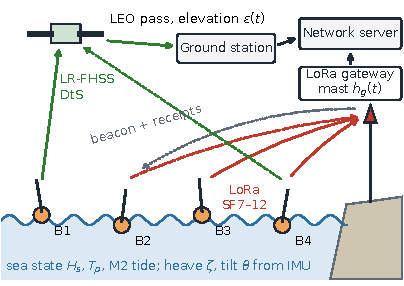
\includegraphics[width=\columnwidth]{figs/fig_network.pdf}
\caption{Network model. Each buoy chooses per epoch between LoRa SF7--SF12 towards a mast gateway, an LR-FHSS frame to a passing LEO satellite, or buffering; wave heave and tilt, tide and ducting modulate the links.}\label{fig:net}
\end{figure}

\subsection{Sea State and Link Models}
The sea is described by the significant wave height $\Hs(t)$ and peak period $T_p(t)$. The heave of a surface-following buoy and its hull tilt are
\begin{equation}
\zeta_n(t)\sim\mathcal{N}\big(0,(\Hs/4)^2\big),\quad
\theta_{\mathrm{rms}}=\kappa_b\frac{\pi \Hs}{\sqrt2\,L_p},\quad L_p=\frac{gT_p^2}{2\pi},\label{eq:heave}
\end{equation}
with hull response $\kappa_b$. The IMU supplies noisy estimates $\Hhat,\hat T_p,\hat\theta_{\mathrm{rms}}$, the only sea-state quantities available on board.

The antenna heights are $h_b=h_0+\zeta_n$ and $h_g(t)=\bar h_g+A_{\mathrm{tide}}\sin(2\pi t/T_{M2}+\phi)$, where the M2 tide ($T_{M2}=12.42$~h) changes the mast height above water. With the direct--reflected phase difference $\Delta\varphi=4\pi h_g h_b/(\lambda d_n)$, sea reflection coefficient $\Gamma\approx-1$, Ament roughness factor $\rho=\exp[-8(\pi\sigma_h\sin\psi/\lambda)^2]$ with $\sigma_h=\Hs/4$ and grazing angle $\psi$, and a diffraction slope $\beta$ beyond the radio horizon $d_h$ \cite{b8,b9}, the path loss is
\begin{equation}
PL=20\log_{10}\tfrac{4\pi d_n}{\lambda}-20\log_{10}\big|1+\Gamma\rho e^{-j\Delta\varphi}\big|+\beta(d_n-d_h)^+ .\label{eq:pl}
\end{equation}
The uplink SNR adds transmit power, the tilted antenna gain $G_b(\theta)$, the gateway gain, AR(1) log-normal shadowing $S$, a ducting gain $D\ge0$, a wave-blockage loss $B$ and Rician fading $F$ whose K-factor falls with $\Hs$:
\begin{equation}
\mathrm{SNR}_L=P_t+G_b(\theta_n)+G_g-PL+S+D-B+F-N_0 .\label{eq:snr}
\end{equation}
A frame with SF$k$ succeeds if $\mathrm{SNR}_L\ge\gamma_k$ and it does not collide; under background load $G$ and time on air $T_k$ \cite{b24},
\begin{equation}
Y_k=\mathbf{1}\{\mathrm{SNR}_L\ge\gamma_k\}\,\mathbf{1}\{\text{no collision}\},\quad \Pr[\text{coll.}]=1-e^{-2GT_k}.\label{eq:success}
\end{equation}
Since $\gamma_7>\dots>\gamma_{12}$, the SNR part of \eqref{eq:success} is nested across SFs, which the predictor exploits.

A LEO satellite at altitude $h_s$ is visible during passes with known elevation $\varepsilon(t)$ and slant range $r(\varepsilon)$. The LR-FHSS margin, with a hemispherical buoy antenna evaluated at the tilt-corrected elevation, is
\begin{equation}
M_S=P_s+G_q(\varepsilon-\theta_n)+G_{\mathrm{sat}}-20\log_{10}\tfrac{4\pi r(\varepsilon)}{\lambda}-L_a-P_{\mathrm{sens}}+F_S ,\label{eq:sat}
\end{equation}
and the frame succeeds if $M_S\ge0$, it survives the Doppler rate at low elevation (probability $1-p_D(\varepsilon)$ \cite{b17}) and it does not collide. The energy of an attempt is $E_a=P_{\mathrm{elec}}(a)T_a$ with $E_\defer=0$; for a 20-byte payload it is 8.5~mJ at SF7, 197.8~mJ at SF12 and 780~mJ for a 2-s LR-FHSS frame, a ratio of almost 1:100.

\begin{table}[!t]
\caption{Main Symbols}\label{tab:sym}
\centering\scriptsize\setlength{\tabcolsep}{3pt}
\begin{tabular}{@{}ll@{}}
\toprule
Symbol & Meaning\\\midrule
$\Hs,T_p;\ \Hhat,\hat\theta_{\mathrm{rms}}$ & sea state; IMU estimates\\
$\zeta,\theta,\kappa_b$ & heave, tilt, hull response\\
$h_b,h_g,A_{\mathrm{tide}}$ & buoy and gateway heights, tidal amplitude\\
$\Gamma,\rho,\beta$ & reflection, roughness factor, diffraction slope\\
$S,D,B,F$ & shadowing, ducting, blockage, fading (dB)\\
$\gamma_k,T_k,E_a$ & SF$k$ threshold, time on air; energy of $a$\\
$\varepsilon,M_S$ & satellite elevation, LR-FHSS margin\\
$Y\in\{0,1\}^7,\ b(x)$ & per-action success; sea-state stratum\\
$\mu_a,\sigma_a,s_a,\kappa$ & ensemble mean, spread, score, penalty\\
$\alpha,\delta,\lambda_b$ & risk target, confidence, stratum threshold\\
$\pi_k,\ell_k$ & physics prior of action $k$, its logit\\
$u_t,g,A_{\max},\alpha_U$ & urgency flag, guard, age limit, urgent target\\
$\gamma$ & adaptive conformal step size\\
\bottomrule
\end{tabular}
\end{table}

\subsection{Problem Statements and Research Gap}
The models above expose five problems. P1: through \eqref{eq:heave}--\eqref{eq:snr} the link budget follows $\Hs$, the tide and ducting, so a fixed SNR margin is too generous in calm water and too optimistic in rough water. P2: action costs differ by two orders of magnitude, and SAT exists only during passes. P3: learned link predictors output uncalibrated scores, so a buoy cannot tell how often it will fail. P4: storms, new sites and hardware changes shift the data after deployment. P5: a reading not delivered within the age limit $A_{\max}$ is lost. Correspondingly, the literature leaves five gaps: learned LoRa adaptation \cite{b25,b26,b27} has no failure bound; motion data \cite{b28} have not conditioned a guarantee or a physical prior; conformal wireless AI \cite{b29,b31} covers prediction sets, not a sequential, cost-ordered choice with a non-monotone loss; per-sea-state guarantees that recover after shift are unstudied; and no scheme allocates reliability by data urgency.

\subsection{Selective Prediction Formulation}
Deferring is the buoy's natural abstention: a buffered reading can ride on the next successful frame. Let $x$ be the inputs available before epoch $t$, $Y\in\{0,1\}^7$ the success indicators of the seven transmit actions, and $b(x)\in\{$calm, moderate, rough$\}$ the stratum given by $\Hhat<1$~m, $1\le\Hhat<2$~m and $\Hhat\ge2$~m. For a policy $\pi$ the attempt-failure loss and per-stratum risk are
\begin{equation}
\ell(\pi;x,Y)=\mathbf{1}\{\pi(x)\neq\defer\}\big(1-Y_{\pi(x)}\big),\quad R_b(\pi)=\mathbb{E}[\ell\mid b(x)=b].\label{eq:loss}
\end{equation}
WARDEN seeks the least-energy policy whose risk meets the target with high confidence over the calibration data:
\begin{equation}
\min_\pi\ \mathbb{E}\big[E_{\pi(x)}\big]\quad\text{s.t.}\quad \Pr\big[R_b(\pi)\le\alpha\big]\ge1-\delta,\ \ \forall b ,\label{eq:problem}
\end{equation}
within the threshold family
\begin{equation}
\pi_{\boldsymbol\lambda}(x)=\min\{a\in\mathcal{A}_t\setminus\{\defer\}:s_a(x)\ge\lambda_{b(x)}\},\label{eq:policy}
\end{equation}
with actions ordered by energy, $\mathcal{A}_t$ excluding SAT outside passes, $\pi_{\boldsymbol\lambda}=\defer$ if the set is empty, and $s_a$ the score of Section~\ref{sec:uq}. Raising $\lambda_b$ moves the choice to more robust actions or to deferral but does not make the loss monotone, because a robust action can still fail on a given draw; this is why LTT \cite{b34} is used rather than conformal risk control for monotone losses \cite{b33}.

\section{Proposed WARDEN Algorithm}\label{sec:alg}
WARDEN has three stages (Fig.~\ref{fig:pipe}): input representation with a physics prior, the attention predictor, and uncertainty- and urgency-aware certified selection. The full system with both extensions is called WARDEN-PI-U.

\begin{figure*}[!t]
\centering
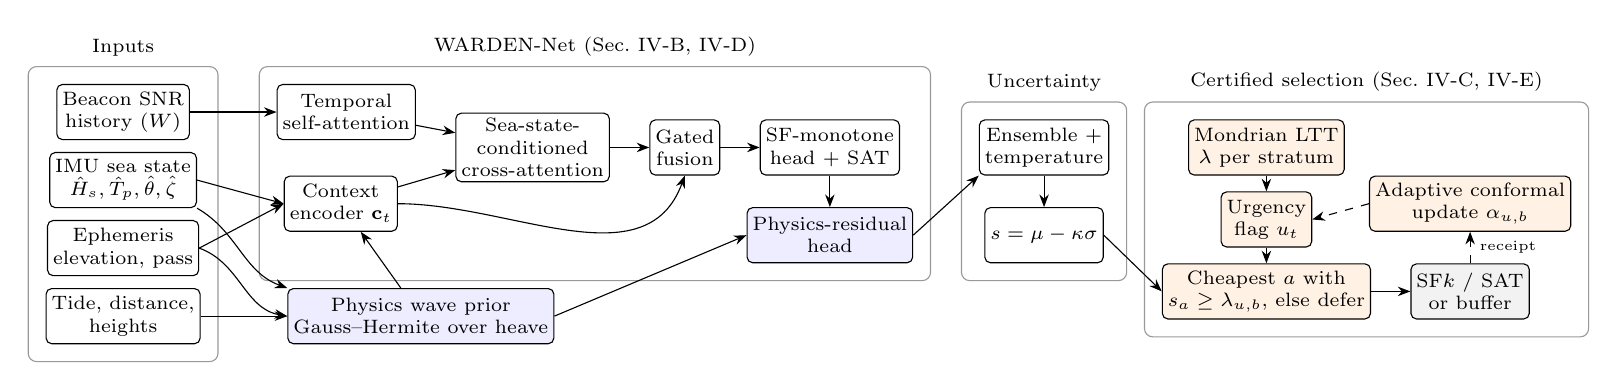
\begin{tikzpicture}[font=\scriptsize, node distance=3mm and 4mm,
  b/.style={draw, rounded corners=2pt, align=center, inner sep=2pt, minimum height=7mm, fill=white},
  phys/.style={b, fill=blue!7}, sel/.style={b, fill=orange!10},
  grp/.style={draw=black!40, rounded corners=3pt, inner sep=2.2mm},
  >={Stealth[length=1.6mm]}]
\node[b] (snr) {Beacon SNR\\history ($W$)};
\node[b, below=1.5mm of snr] (imu) {IMU sea state\\$\hat H_s,\hat T_p,\hat\theta,\hat\zeta$};
\node[b, below=1.5mm of imu] (eph) {Ephemeris\\elevation, pass};
\node[b, below=1.5mm of eph] (geo) {Tide, distance,\\heights};
\node[b, right=11mm of snr] (sa) {Temporal\\self-attention};
\node[b, right=11mm of imu, yshift=-3mm] (ctx) {Context\\encoder $\mathbf{c}_t$};
\node[phys, right=11mm of geo] (prior) {Physics wave prior\\Gauss--Hermite over heave};
\node[b, right=5mm of sa, yshift=-4.5mm] (xa) {Sea-state-\\conditioned\\cross-attention};
\node[b, right=5mm of xa] (gf) {Gated\\fusion};
\node[b, right=5mm of gf] (head) {SF-monotone\\head $+$ SAT};
\node[phys, below=4mm of head] (res) {Physics-residual\\head};
\node[b, right=10mm of head] (ens) {Ensemble $+$\\temperature};
\node[b, below=4mm of ens] (score) {$s=\mu-\kappa\sigma$};
\node[sel, right=10mm of ens] (ltt) {Mondrian LTT\\$\lambda$ per stratum};
\node[sel, below=2mm of ltt] (urg) {Urgency\\flag $u_t$};
\node[sel, below=2mm of urg] (rule) {Cheapest $a$ with\\$s_a\ge\lambda_{u,b}$, else defer};
\node[b, fill=black!5, right=5mm of rule] (out) {SF$k$ / SAT\\or buffer};
\node[sel, above=4mm of out] (aci) {Adaptive conformal\\update $\alpha_{u,b}$};
\begin{scope}[on background layer]
\node[grp, fit=(snr)(geo), label={[font=\scriptsize]above:Inputs}] {};
\node[grp, fit=(sa)(ctx)(xa)(gf)(head)(res), label={[font=\scriptsize]above:WARDEN-Net (Sec.~IV-B, IV-D)}] {};
\node[grp, fit=(ens)(score), label={[font=\scriptsize]above:Uncertainty}] {};
\node[grp, fit=(ltt)(rule)(out)(aci), label={[font=\scriptsize]above:Certified selection (Sec.~IV-C, IV-E)}] {};
\end{scope}
\draw[->] (snr) -- (sa); \draw[->] (imu.east) -- (ctx.west); \draw[->] (eph.east) -- (ctx.west);
\draw[->] (geo) -- (prior); \draw[->] (imu.south east) to[out=-30,in=160] (prior.north west); \draw[->] (eph.east) to[out=-20,in=170] (prior.west);
\draw[->] (prior) -- (ctx); \draw[->] (sa) -- (xa); \draw[->] (ctx) -- (xa); \draw[->] (xa) -- (gf);
\draw[->] (ctx.east) to[out=0,in=-110] (gf.south); \draw[->] (gf) -- (head); \draw[->] (head) -- (res);
\draw[->] (prior.east) -- (res.west); \draw[->] (res.east) -- (ens.south west); \draw[->] (ens) -- (score);
\draw[->] (score.east) -- (rule.west); \draw[->] (ltt) -- (urg); \draw[->] (urg) -- (rule); \draw[->] (rule) -- (out);
\draw[->, dashed] (out) -- node[right, font=\tiny]{receipt} (aci); \draw[->, dashed] (aci.west) -- (urg.east);
\end{tikzpicture}
\caption{WARDEN-PI-U pipeline: inputs, physics wave prior, WARDEN-Net with physics-residual head, ensemble uncertainty, and urgency-aware selection with offline Mondrian LTT and online adaptive conformal updates driven by the receipt bitmap.}\label{fig:pipe}
\end{figure*}

\subsection{Preprocessing, Segmentation and Input Representation}
Each buoy stream is cut into sliding windows of $W=16$ epochs (2~h 40~min), long enough to span the shadowing decorrelation time and one fifth of a tidal cycle; windows end at the beacon of epoch $t$, so nothing from the decision interval leaks into the input. Each step carries $\mathbf{u}_\tau=[\mathrm{SNR}^{\mathrm{bcn}}_\tau/10,m_\tau,\hat H_{s,\tau},\hat T_{p,\tau}/10,\hat\theta_{\mathrm{rms},\tau}/10,\hat\zeta_\tau,\varepsilon_\tau/90]$, where $m_\tau$ flags a lost beacon. The context $\mathbf{c}_t$ holds distance, antenna height, current sea state, elevation and visibility, time of day as $(\sin,\cos)$ and epochs to the next pass. Features are standardized with training statistics only.

\subsection{Attention-Enhanced Architecture (WARDEN-Net)}
The window $\mathbf{U}\in\mathbb{R}^{W\times7}$ is embedded with a learned positional code $\mathbf{P}$ and passed through one post-norm Transformer block with $H=2$ heads and width $d=32$:
\begin{equation}
\mathbf{Z}_1=\mathrm{LN}\big(\mathbf{Z}_0+\mathrm{MHA}(\mathbf{Z}_0,\mathbf{Z}_0)\big),\ \ \mathbf{Z}=\mathrm{LN}\big(\mathbf{Z}_1+\mathrm{FFN}(\mathbf{Z}_1)\big),\label{eq:enc}
\end{equation}
with $\mathbf{Z}_0=\mathbf{U}\mathbf{W}_e+\mathbf{P}$. The context, encoded as $\mathbf{e}=\mathrm{GELU}(\mathbf{c}\mathbf{W}_{c1})\mathbf{W}_{c2}$, is the \emph{query} of a sea-state-conditioned cross-attention over the history, followed by a gate that decides how much history to trust:
\begin{equation}
\mathbf{z}=\mathrm{MHA}(\mathbf{e},\mathbf{Z}),\quad \mathbf{v}=\mathrm{GELU}\big([\mathbf{z}\odot\sigma(\mathbf{e}\mathbf{W}_g+\mathbf{b}_g)+\mathbf{e}]\mathbf{W}_h\big).\label{eq:cross}
\end{equation}
In calm water the query can emphasize the latest beacons, which track slow shadowing and ducting; in rough water it can spread weight to average out wave-induced fluctuations. Following the nesting of \eqref{eq:success}, an SF-monotone ordinal head builds the SF logits from a base logit and non-negative increments, with a separate satellite logit:
\begin{equation}
z_7=\mathbf{v}^\top\mathbf{w}_0,\ \ z_k=z_7+\textstyle\sum_{j=8}^{k}\mathrm{softplus}(\mathbf{v}^\top\mathbf{w}_j),\ \ z_{\mathrm S}=\mathbf{v}^\top\mathbf{w}_{\mathrm S},\label{eq:head}
\end{equation}
so $p_7\le\dots\le p_{12}$ by construction. All outputs are trained jointly with a binary cross-entropy in which the satellite term is masked outside passes. In the testbed every action is labeled by counterfactual simulation; in deployment the labels come from probe frames during commissioning.

\subsection{Uncertainty Estimation, Calibration and Risk-Controlled Selection}\label{sec:uq}
An ensemble of $M=3$ networks is trained; each member's logits are divided by an action-specific temperature fitted on validation data, giving mean $\mu_a(x)$ and spread $\sigma_a(x)$ of the calibrated probabilities. Disagreement becomes caution through the lower-confidence score
\begin{equation}
s_a(x)=\mathrm{clip}\big(\mu_a(x)-\kappa\sigma_a(x),0,1\big),\quad\kappa=1.\label{eq:score}
\end{equation}
\emph{Mondrian LTT.} Let stratum $b$ hold $n_b$ calibration epochs and $\Lambda=\{\lambda_1>\dots>\lambda_J\}$ be a grid from 0.999 to 0.30 ($J=141$). For each $\lambda_j$ the empirical risk $\hat R_b(\lambda_j)$ of \eqref{eq:policy} gives the exact binomial p-value for $H_{b,j}\!:R_b(\lambda_j)>\alpha$,
\begin{equation}
p_{b,j}=\Pr\big[\mathrm{Bin}(n_b,\alpha)\le n_b\hat R_b(\lambda_j)\big],\label{eq:pval}
\end{equation}
and fixed-sequence testing from the most conservative threshold yields
\begin{equation}
\hat\lambda_b=\lambda_{\hat j},\quad \hat j=\max\{j: p_{b,1}\le\delta,\dots,p_{b,j}\le\delta\},\label{eq:lambda}
\end{equation}
with $\hat\lambda_b=1.01$ (always defer) if $p_{b,1}>\delta$.

\emph{Proposition 1:} If calibration and test epochs are exchangeable within each stratum and the predictor is fixed before calibration, then $\Pr[R_b(\pi_{\hat\lambda_b})\le\alpha]\ge1-\delta$ for every $b$.

\emph{Proof sketch:} Fixed-sequence testing at level $\delta$ controls the family-wise error rate without monotonicity, because a false rejection can occur only at the first true null \cite{b34}; \eqref{eq:pval} is valid because $n_b\hat R_b$ is binomial with parameter $R_b$; conditioning on $b$ is a Mondrian partition that preserves exchangeability within each cell. \hfill$\square$

\emph{Online update.} Storms and site changes break exchangeability. Each stratum keeps a working level $\alpha_{b,t}$, maps it to the most aggressive threshold whose calibration risk curve stays below it, and corrects it with the realized loss $\mathrm{err}_t$ read from the receipt bitmap:
\begin{equation}
\alpha_{b,t+1}=\mathrm{clip}\big(\alpha_{b,t}+\gamma(\alpha-\mathrm{err}_t),10^{-4},0.5\big),\ \ \gamma=0.005 .\label{eq:aci}
\end{equation}
Without clipping, the long-run failure frequency in each stratum converges to $\alpha$ at rate $O(1/T_b)$ for any data sequence \cite{b35}.

\subsection{Physics-Informed Wave Prior and Residual Head (WARDEN-PI)}
The buoy knows $d_n$, $h_0$, $\bar h_g$, the tide table, its IMU sea state and the ephemeris, which suffice to evaluate the deterministic part of \eqref{eq:pl}--\eqref{eq:sat}. Let $\overline{\mathrm{SNR}}(\zeta)$ be \eqref{eq:snr} without shadowing, ducting and fading, at heave $\zeta$, mean tilt and roughness $\Hhat/4$. Integrating \eqref{eq:heave} with $Q=10$ Gauss--Hermite nodes $\xi_q$ and weights $w_q$ gives the wave-averaged prior of SF$k$,
\begin{equation}
\pi_k=\sum_{q=1}^{Q}w_q\Big[(1-p_B)\Phi\Big(\tfrac{\overline{\mathrm{SNR}}_q-\gamma_k}{\sigma_r}\Big)+p_B\Phi\Big(\tfrac{\overline{\mathrm{SNR}}_q-L_B-\gamma_k}{\sigma_r}\Big)\Big],\label{eq:prior}
\end{equation}
with $\overline{\mathrm{SNR}}_q=\overline{\mathrm{SNR}}(\xi_q\Hhat/4)$, residual spread $\sigma_r=4.5$~dB, blockage loss $L_B$ and blockage probability $p_B$ implied by $\Hhat$ and $h_0$ \cite{b8}. The satellite prior is $\pi_{\mathrm S}=\mathbf{1}\{\varepsilon>0\}\Phi(M_S/\sigma_s)(1-p_D)(1-p_c)$. The prior logits $\ell_k$ are appended to $\mathbf{c}_t$, so the cross-attention query is physics-informed, and they enter a physics-residual head
\begin{equation}
\tilde z_k=z_k+\mathrm{softplus}(\beta_{\mathrm{SF}})\,\ell_k,\qquad \tilde z_{\mathrm S}=z_{\mathrm S}+\mathrm{softplus}(\beta_{\mathrm S})\,\ell_{\mathrm S},\label{eq:residual}
\end{equation}
with learnable scalars. A shared $\beta_{\mathrm{SF}}$ keeps the SF ordering, and the network learns only what physics leaves unexplained; if the prior is wrong, $\beta$ can shrink and certification still enforces the target. Evaluating \eqref{eq:prior} costs about $10^3$ operations per epoch.

\subsection{Urgency-Aware Mondrian Certification (WARDEN-U)}
A reading close to the age limit is lost if the buoy keeps deferring. WARDEN-U refines the Mondrian partition with the flag $u_t=\mathbf{1}\{t-t^{\mathrm{old}}_n\ge A_{\max}-g\}$, where $t^{\mathrm{old}}_n$ is the arrival of the oldest buffered reading and $g=3$ a guard. Each cell $(u,b)$ keeps its own level and target,
\begin{equation}
\alpha_{u,b,t+1}=\mathrm{clip}\big(\alpha_{u,b,t}+\gamma(\alpha^{(u)}-\mathrm{err}_t),10^{-4},0.6\big),\label{eq:urgent}
\end{equation}
with $\alpha^{(0)}=\alpha$ and $\alpha^{(1)}=\alpha_U$, so ordinary traffic converges to $\alpha$, urgent traffic to $\alpha_U$, and the overall risk is the mixture $R=(1-\rho_U)R^{(0)}+\rho_U R^{(1)}$ with $\rho_U=\Pr[u_t=1]$. Even with $\alpha_U=\alpha$ the split helps, because the update no longer averages the different failure statistics of fresh and nearly expired buffers. Algorithm~\ref{alg:online} summarizes on-board operation.

\begin{algorithm}[!t]
\caption{WARDEN-PI-U Operation on Buoy $n$}\label{alg:online}
\footnotesize
\begin{algorithmic}[1]
\Require ensemble, temperatures, risk curves $\hat R_b(\cdot)$ from Mondrian LTT; $\alpha,\alpha_U,\gamma,g$
\State $\alpha_{u,b}\gets\alpha$ ($u=0$) or $\alpha_U$ ($u=1$) for all cells
\For{each epoch $t$}
\State receive beacon; read SNR and receipt bit $\mathrm{err}_{t-1}$; update the previous cell by \eqref{eq:urgent}
\State build window and context; compute prior by \eqref{eq:prior}
\State $b\gets$ stratum$(\Hhat)$; $u\gets u_t$
\State $\lambda\gets$ most aggressive $\lambda_j$ with $\hat R_b(\lambda_1..\lambda_j)\le\alpha_{u,b}$
\State compute $s_a$ by \eqref{eq:score}, \eqref{eq:residual} for available actions
\State $a^\star\gets$ cheapest $a$ with $s_a\ge\lambda$, else $\defer$
\State \textbf{if} $a^\star=\defer$ buffer reading (drop ages $>A_{\max}$) \textbf{else} send buffer with $a^\star$
\EndFor
\end{algorithmic}
\end{algorithm}

\emph{Complexity.} WARDEN-Net has 17\,487 parameters; a forward pass costs $O(W^2d+Wd^2)\approx10^5$ multiply--accumulates, so the three-member ensemble needs under 1~MFLOP per decision, within reach of a Cortex-M4-class microcontroller every 10~min. The online update is one table look-up and one addition.

\begin{figure}[!t]
\centering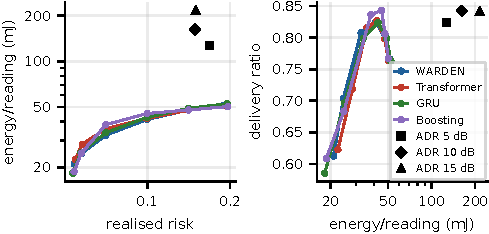
\includegraphics[width=\columnwidth]{figs/fig_tradeoff.pdf}
\caption{Trade-offs for $\alpha\in\{0.01,\dots,0.20\}$ with Mondrian LTT and online update, against ADR with 5-, 10- and 15-dB margins (mean of three seeds).}\label{fig:tradeoff}
\end{figure}

\begin{figure*}[!t]
\centering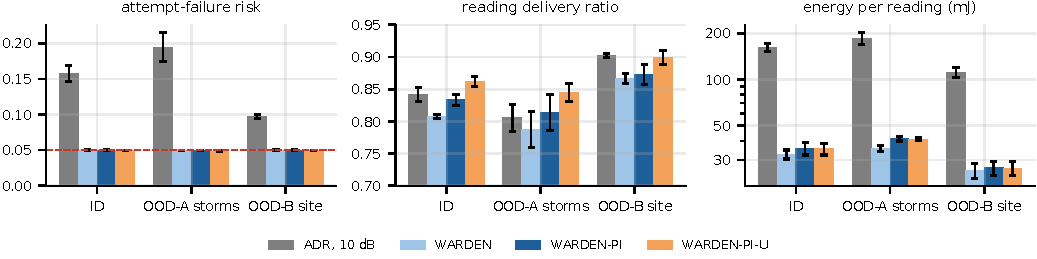
\includegraphics[width=\textwidth]{figs/fig_results.pdf}
\caption{Attempt-failure risk, reading delivery ratio and energy per reading of ADR-10 and the WARDEN variants in distribution and under the two shifts ($\alpha=\alpha_U=0.05$; error bars: standard deviation over three seeds; dashed line: $\alpha$).}\label{fig:res}
\end{figure*}

\section{Experimental Setup}\label{sec:setup}
\emph{Testbed.} All experiments run in an open software testbed (Python, NumPy, SciPy, scikit-learn and a purpose-written automatic-differentiation engine) that implements Section~\ref{sec:model}; it is a physics-guided emulator, not a sea trial, with parameters taken from published offshore and DtS studies \cite{b5,b8,b15,b16,b17,b18,b19} (Table~\ref{tab:param}). Each deployment has 20 buoys at 5--32~km with antennas at 0.8--1.5~m, observed for 60 days at 10-min epochs. The regional sea state follows a log-AR(1) process with Poisson storms. For every epoch the true success probability of every action is computed from 32 Monte Carlo draws of wave phase, blockage and fading, and one draw gives the labels.

\begin{table}[!t]
\caption{Testbed Parameters}\label{tab:param}
\centering\scriptsize\setlength{\tabcolsep}{3pt}
\begin{tabular}{@{}ll@{}}
\toprule
Parameter & Value\\\midrule
Carrier, bandwidth, noise figure & 868 MHz, 125 kHz, 6 dB\\
LoRa power, gateway gain, mast & 14 dBm, 6 dBi, 15 m (10 m in OOD-B)\\
Tide; diffraction slope & M2, 1.5 m; 1.2 dB/km\\
Shadowing; ducting & AR(1) $\rho{=}0.97$, 3 dB; 0--6 dB\\
SF thresholds $\gamma_7..\gamma_{12}$ & $-7.5$ to $-20$ dB in 2.5-dB steps\\
LEO altitude, mean revisit & 550 km, 95 min\\
LR-FHSS power, sensitivity, frame & 22 dBm, $-137$ dBm, 2.0 s\\
Radio power (14/22 dBm) & 0.15 W / 0.39 W\\
Payload, epoch, age limit $A_{\max}$ & 20 B, 10 min, 3 h\\
Sea state ID / OOD-A & mean $\Hs$ 1.2/1.8 m, storm peak 2.5--3.5/4--7 m\\
\bottomrule
\end{tabular}
\end{table}

\emph{Splits and shifts.} Splits are chronological: days 0--36 for training, 36--42 for validation and temperatures, 42--48 for calibration and 48--60 for testing. OOD-A is a new deployment with severe storms; OOD-B is a site and hardware shift with a lower mast, a livelier hull, heavier interference and shorter distances. Every experiment uses three seeds, which change the deployment, the initialization and the calibration draw; we report means, with standard deviations where they matter.

\emph{Baselines.} Rule-based: ADR-$m$, which picks the smallest SF whose threshold plus a margin $m\in\{5,10,15\}$~dB lies below a smoothed beacon SNR, otherwise SAT if visible, otherwise SF12; always-SF12; satellite-first; and an oracle that picks the cheapest action that actually succeeds. Predictors, all followed by the same calibration and selection: logistic regression, histogram gradient boosting and an MLP on 42 engineered features, a GRU, and a Transformer encoder representative of \cite{b20,b21,b22}. Physics-informed: the prior \eqref{eq:prior} alone with certification, and gradient boosting given the prior as features. Selection rules: thresholds 0.5 and $1-\alpha$, global LTT, Mondrian LTT, with the update \eqref{eq:aci}, and with urgency cells. To test a wrong model, WARDEN-PI is also run with a biased prior ($\Gamma=-0.80$ instead of $-0.95$, 0.8 instead of 1.2~dB/km, a 3-m mast error, 3-dB spread, 6-dB blockage and a 2-dB optimistic satellite receiver).

\emph{Metrics.} AUROC, Brier score and expected calibration error (ECE) measure prediction; the realized attempt-failure risk (overall and per stratum), deferral, reading delivery ratio (RDR, readings delivered within $A_{\max}$), latency and energy per delivered reading measure decisions. Unless stated, $\alpha=0.05$ and $\delta=0.1$.

\section{Results}\label{sec:results}
\subsection{Prediction Quality}
All predictors reach similar discrimination in distribution (AUROC 0.883--0.886) because much of the remaining uncertainty is aleatoric. WARDEN-Net has the lowest Brier score in distribution (0.0839) and under storms (0.0930), and under the site shift its ECE (0.023) is below that of the Transformer (0.032), gradient boosting (0.028) and the MLP (0.036), close to the GRU (0.021). These differences are small; the value of the architecture lies in ordered, calibrated scores for the selection layer rather than in raw accuracy.

\subsection{Certified Link Selection}
Table~\ref{tab:main} reports decisions in distribution. Rule-based policies never defer but fail often: ADR with a 10-dB margin fails 15.8\% of its attempts and 25.1\% in rough water, and other margins only move the energy. Uncertainty-unaware thresholds show two failure modes: 0.5 fails 16.7\% of the time, whereas $1-\alpha$ defers over half the epochs and delivers only 58.3\% of readings. Global LTT overshoots in rough water (0.053) because its single threshold is dominated by calm data; Mondrian LTT stays within the $\delta$ allowance, and the online update brings the risk to 0.050 in every stratum and seed. The base WARDEN then spends 32.6~mJ per reading, five times less than ADR-10 (162.5~mJ), but delivers 3.4 points fewer readings. WARDEN-PI-U removes this penalty: it delivers 86.2\% of readings, above ADR-10 (84.2\%), at 35.3~mJ. Ordinary traffic fails at exactly 5.0\%; urgent epochs, about 6\% of all, fail at 3.3\% because their own level adapts to the conditions in which buffers near expiry.

\begin{table}[!t]
\caption{Link Selection in Distribution ($\alpha=0.05$, $\delta=0.1$, Mean of Three Seeds)}\label{tab:main}
\centering\scriptsize\setlength{\tabcolsep}{2.4pt}
\begin{tabular}{@{}lccccccc@{}}
\toprule
Policy & Risk & Calm & Mod. & Rough & Defer & RDR & mJ\\\midrule
ADR, 10 dB & 0.158 & 0.088 & 0.138 & 0.251 & 0 & 0.842 & 162.5\\
Always SF12 & 0.172 & 0.114 & 0.154 & 0.255 & 0 & 0.828 & 239.1\\
Satellite first & 0.202 & 0.152 & 0.185 & 0.271 & 0 & 0.798 & 396.8\\
Net, thr. 0.5 & 0.167 & 0.118 & 0.154 & 0.225 & 0.103 & 0.779 & 54.3\\
Net, thr. $1-\alpha$ & 0.012 & 0.012 & 0.015 & 0.009 & 0.523 & 0.583 & 20.8\\
Net, global LTT & 0.046 & 0.036 & 0.051 & 0.053 & 0.297 & 0.804 & 31.5\\
Net, Mondrian LTT & 0.044 & 0.035 & 0.051 & 0.048 & 0.302 & 0.798 & 31.4\\
WARDEN & 0.050 & 0.050 & 0.050 & 0.050 & 0.293 & 0.808 & 32.6\\
\textbf{WARDEN-PI-U} & \textbf{0.049} & -- & -- & -- & -- & \textbf{0.862} & 35.3\\
Oracle (bound) & 0 & 0 & 0 & 0 & 0.111 & 0.998 & 39.2\\
\bottomrule
\end{tabular}
\end{table}

Fig.~\ref{fig:tradeoff} varies $\alpha$ from 0.01 to 0.20. Certified policies use 3--8 times less energy per reading than the ADR family across the range. The delivery ratio peaks near $\alpha=0.10$ and then falls, because each failed unconfirmed frame destroys the whole buffer it carries. At the risk that ADR-10 incurs on the calibration days (0.166), WARDEN matches it with 3.3 times less energy. The certification layer is model agnostic: gradient boosting gives a 2.9-point higher RDR than WARDEN-Net at 17\% more energy, and either can be certified.



\subsection{Physics Prior, Urgency Cells and Distribution Shift}
Fig.~\ref{fig:res} and Table~\ref{tab:shift} compare the variants under the online certificate. Every certified policy holds the risk at 0.049--0.050 in all scenarios, whereas ADR-10 fails 9.7--19.5\% of its attempts. With full training data the physics-residual head barely changes the Brier score (0.0842 vs.\ 0.0839) but improves decisions: WARDEN-PI raises the RDR from 0.808 to 0.834 in distribution, from 0.788 to 0.813 under storms and from 0.866 to 0.873 after the site shift. The urgency cells give the largest gain: WARDEN-PI-U delivers 86.2\%, 84.5\% and 90.0\% of readings in the three scenarios, exceeding ADR-10 in distribution and under storms (80.5\%) and matching it after the site shift (90.3\%), with 4.2--4.6 times less energy. Gradient boosting reaches 0.837 in distribution; giving it the prior as features does not help (0.834), so the benefit of the prior is tied to the residual design \eqref{eq:residual}. Raising $\alpha_U$ above $\alpha$ is counter-productive: at $\alpha_U=0.30$ the RDR falls to 0.825 because failed urgent frames destroy full buffers, so $\alpha_U=\alpha$ is recommended.



\begin{table}[!t]
\caption{Behavior Under Distribution Shift ($\alpha=\alpha_U=0.05$)}\label{tab:shift}
\centering\scriptsize\setlength{\tabcolsep}{3pt}
\begin{tabular}{@{}llcccc@{}}
\toprule
Scenario & Policy & Risk & Rough & RDR & mJ\\\midrule
\multirow{4}{*}{OOD-A storms} & ADR, 10 dB & 0.195 & 0.266 & 0.805 & 185.9\\
& Net, Mondrian LTT & 0.038 & 0.037 & 0.743 & 32.9\\
& WARDEN & 0.050 & 0.050 & 0.788 & 35.6\\
& \textbf{WARDEN-PI-U} & \textbf{0.049} & -- & \textbf{0.845} & 40.9\\\midrule
\multirow{5}{*}{OOD-B site} & ADR, 10 dB & 0.097 & 0.165 & 0.903 & 111.2\\
& Transformer, Mondrian LTT & 0.063 & 0.063 & 0.887 & 30.8\\
& Net, Mondrian LTT & 0.052 & 0.055 & 0.869 & 26.7\\
& WARDEN & 0.050 & 0.050 & 0.866 & 25.5\\
& \textbf{WARDEN-PI-U} & \textbf{0.049} & -- & \textbf{0.900} & 26.5\\
\bottomrule
\end{tabular}
\end{table}

Under storms the offline certificate stays valid but becomes conservative (0.038), and the online update recovers the unused budget. The site shift changes the conditional relation between features and outcomes, so the offline certificate is violated by every predictor that does not defer heavily (0.052--0.067); the online update restores 0.050 within about one day (Fig.~\ref{fig:online}).

\begin{figure}[!t]
\centering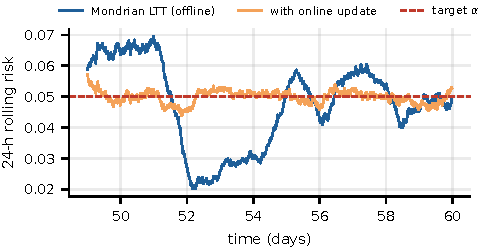
\includegraphics[width=\columnwidth]{figs/fig_online.pdf}
\caption{24-h rolling risk after the site shift (OOD-B, seed 1).}\label{fig:online}
\end{figure}

\subsection{Commissioning With Little Data}
Fig.~\ref{fig:low} trains on only 2, 4 or 8 days. Here the prior pays off clearly: with two days WARDEN-PI lowers the Brier score from 0.0958 to 0.0908 and WARDEN-PI-U delivers 84.8\% of readings, above ADR-10, gradient boosting (80.7\%) and the prior alone (80.9\%), at 29~mJ instead of 162~mJ. The risk stays at 0.049--0.052 throughout, because the guarantee does not depend on predictor quality; only efficiency does.

\begin{figure}[!t]
\centering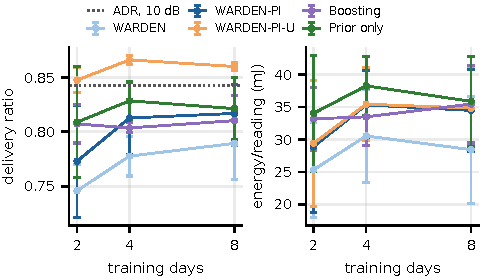
\includegraphics[width=\columnwidth]{figs/fig_lowdata.pdf}
\caption{Delivery ratio and energy per reading versus days of labeled training data ($\alpha=0.05$; error bars: standard deviation over three seeds).}\label{fig:low}
\end{figure}

\subsection{Ablation, Robustness and Prior Misspecification}
Table~\ref{tab:abl} isolates each component under offline Mondrian LTT. Removing the IMU features or the uncertainty penalty makes the policy more conservative and unstable across seeds (deferral 0.39 and 0.38 instead of 0.30), because the calm-stratum risk curve becomes ragged and fixed-sequence testing stops early. Removing cross-attention raises the OOD-B risk from 0.052 to 0.063, and removing the monotone head costs 9\% energy. The learned cross-attention concentrates on recent beacons in calm water and flattens in rough water, as intended. With IMU noise raised from 8\% to 30\% or beacon noise from 1 to 3~dB, the online certificate still holds 0.050. With only 250 calibration epochs, 3.3\% of 60 random draws violated the target, below $\delta=10\%$; from 500 epochs no draw did. With the misspecified prior, the risk stays at 0.045--0.050 in all scenarios while the ECE rises to 0.19--0.21 under shift and energy roughly doubles (OOD-A: 73.6 vs.\ 41.1~mJ): a wrong physics model costs energy, not reliability.

\begin{table}[!t]
\caption{Ablation With Offline Mondrian LTT ($\alpha=0.05$)}\label{tab:abl}
\centering\scriptsize\setlength{\tabcolsep}{3pt}
\begin{tabular}{@{}lccccc@{}}
\toprule
Variant & Defer & RDR & mJ & Risk (B) & ECE (B)\\\midrule
WARDEN-Net, full & 0.302 & 0.798 & 31.4 & 0.052 & 0.023\\
w/o IMU features & 0.390 & 0.748 & 28.5 & 0.055 & 0.023\\
w/o cross-attention & 0.305 & 0.807 & 32.8 & 0.063 & 0.038\\
w/o SF-monotone head & 0.292 & 0.797 & 34.2 & 0.056 & 0.027\\
single network & 0.302 & 0.799 & 33.0 & 0.054 & 0.026\\
no penalty ($\kappa=0$) & 0.377 & 0.752 & 30.4 & -- & --\\
\bottomrule
\end{tabular}
\end{table}

\section{Discussion and Limitations}
WARDEN turns link reliability into a design parameter: the operator sets one target $\alpha$ and obtains it per sea state on every buoy, while delivering at least as many readings as an ADR-style rule for about a quarter of the energy, which for a battery-limited buoy translates almost directly into service life. No change to LoRaWAN or LR-FHSS radios is needed, only a beacon with a receipt bitmap, a tide table and a small on-board model. The limitations are concrete. All results come from a synthetic testbed whose propagation family is shared by the prior; the misspecification study bounds the damage, but sea trials are required. Labels for all actions need probe frames in practice, ordinary deliveries wait about 15~min on average, and the online guarantee is a long-run average that does not bound short failure bursts.

\section{Conclusion}
This article presented WARDEN, a decision engine that lets an ocean buoy choose among LoRa spreading factors, a DtS LR-FHSS frame and buffering with a certified bound on attempt failures. It combines a wave-averaged physics prior driven by the buoy's IMU, a sea-state-conditioned attention network with a monotone and physics-residual head, per-sea-state Learn-then-Test calibration and urgency-aware adaptive conformal updates. In a 60-day, 20-buoy testbed with storm and site shifts, it held the failure rate at 5\% in every sea state, delivered 84.5--90.0\% of readings and used 4.2--4.6 times less energy than an ADR rule that failed 10--20\% of its attempts, even with a wrong physics model and two days of training data. Future work will validate WARDEN at sea, learn from bandit feedback, bound failure bursts and add multi-gateway and NB-IoT non-terrestrial links. Code and data generators are available at \url{https://github.com/iitrky/warden}.

\begin{thebibliography}{99}
\footnotesize
\bibitem{b1} T.~Xia, M.~M. Wang, J.~Zhang, and L.~Wang, ``Maritime Internet of Things: Challenges and solutions,'' \emph{IEEE Wireless Commun.}, vol.~27, no.~2, pp.~188--196, 2020, doi: 10.1109/MWC.001.1900322.

\bibitem{b2} F.~S. Alqurashi, A.~Trichili, N.~Saeed, B.~S. Ooi, and M.-S. Alouini, ``Maritime communications: A survey on enabling technologies, opportunities, and challenges,'' \emph{IEEE Internet Things J.}, vol.~10, no.~4, pp.~3525--3547, 2023, doi: 10.1109/JIOT.2022.3219674.

\bibitem{b3} T.~Wei, W.~Feng, Y.~Chen, C.-X. Wang, N.~Ge, and J.~Lu, ``Hybrid satellite-terrestrial communication networks for the maritime Internet of Things: Key technologies, opportunities, and challenges,'' \emph{IEEE Internet Things J.}, vol.~8, no.~11, pp.~8910--8934, 2021, doi: 10.1109/JIOT.2021.3056091.

\bibitem{b4} M.~Jahanbakht, W.~Xiang, L.~Hanzo, and M.~Rahimi Azghadi, ``Internet of underwater things and big marine data analytics: A comprehensive survey,'' \emph{IEEE Commun. Surveys Tuts.}, vol.~23, no.~2, pp.~904--956, 2021, doi: 10.1109/COMST.2021.3053118.

\bibitem{b5} L.~Parri, S.~Parrino, G.~Peruzzi, and A.~Pozzebon, ``Offshore LoRaWAN networking: Transmission performances analysis under different environmental conditions,'' \emph{IEEE Trans. Instrum. Meas.}, vol.~70, pp.~1--10, 2021, doi: 10.1109/TIM.2020.3031193.

\bibitem{b36} L.~Parri, S.~Parrino, G.~Peruzzi, and A.~Pozzebon, ``Low power wide area networks (LPWAN) at sea: Performance analysis of offshore data transmission by means of LoRaWAN connectivity for marine monitoring applications,'' \emph{Sensors}, vol.~19, no.~14, Art. no.~3239, 2019, doi: 10.3390/s19143239.

\bibitem{b6} M.~Centenaro, C.~E. Costa, F.~Granelli, C.~Sacchi, and L.~Vangelista, ``A survey on technologies, standards and open challenges in satellite IoT,'' \emph{IEEE Commun. Surveys Tuts.}, vol.~23, no.~3, pp.~1693--1720, 2021, doi: 10.1109/COMST.2021.3078433.

\bibitem{b7} O.~Kodheli \emph{et al.}, ``Satellite communications in the new space era: A survey and future challenges,'' \emph{IEEE Commun. Surveys Tuts.}, vol.~23, no.~1, pp.~70--109, 2021, doi: 10.1109/COMST.2020.3028247.

\bibitem{b8} Y.~Huo, X.~Dong, and S.~Beatty, ``Cellular communications in ocean waves for maritime Internet of Things,'' \emph{IEEE Internet Things J.}, vol.~7, no.~10, pp.~9965--9979, 2020, doi: 10.1109/JIOT.2020.2988634.

\bibitem{b9} Y.~He \emph{et al.}, ``A novel 3D non-stationary maritime wireless channel model,'' \emph{IEEE Trans. Commun.}, vol.~70, no.~3, p.~2102, 2022, doi: 10.1109/TCOMM.2021.3134275.

\bibitem{b10} Y.~Liu, C.-X. Wang, H.~Chang, Y.~He, and J.~Bian, ``A novel non-stationary 6G UAV channel model for maritime communications,'' \emph{IEEE J. Sel. Areas Commun.}, vol.~39, no.~10, pp.~2992--3005, 2021, doi: 10.1109/JSAC.2021.3088664.

\bibitem{b11} H.~Zhang \emph{et al.}, ``Statistical modeling of evaporation duct channel for maritime broadband communications,'' \emph{IEEE Trans. Veh. Technol.}, vol.~71, no.~10, p.~10228, 2022, doi: 10.1109/TVT.2022.3187753.

\bibitem{b12} L.~Robinson, T.~Newe, J.~Burke, and D.~Toal, ``A simulated and experimental analysis of evaporation duct effects on microwave communications in the Irish Sea,'' \emph{IEEE Trans. Antennas Propag.}, vol.~70, no.~6, 2022, doi: 10.1109/TAP.2022.3145460.

\bibitem{b13} X.~Fang \emph{et al.}, ``NOMA-based hybrid satellite-UAV-terrestrial networks for 6G maritime coverage,'' \emph{IEEE Trans. Wireless Commun.}, vol.~22, no.~1, pp.~138--152, 2023, doi: 10.1109/TWC.2022.3191719.

\bibitem{b14} X.~Li, W.~Feng, J.~Wang, Y.~Chen, N.~Ge, and C.-X. Wang, ``Enabling 5G on the ocean: A hybrid satellite-UAV-terrestrial network solution,'' \emph{IEEE Wireless Commun.}, vol.~27, no.~6, pp.~116--121, 2020, doi: 10.1109/MWC.001.2000076.

\bibitem{b15} G.~Boquet, P.~Tuset-Peir\'o, F.~Adelantado, T.~Watteyne, and X.~Vilajosana, ``LR-FHSS: Overview and performance analysis,'' \emph{IEEE Commun. Mag.}, vol.~59, no.~3, pp.~30--36, 2021, doi: 10.1109/MCOM.001.2000627.

\bibitem{b16} M.~A. Ullah, K.~Mikhaylov, and H.~Alves, ``Analysis and simulation of LoRaWAN LR-FHSS for direct-to-satellite scenario,'' \emph{IEEE Wireless Commun. Lett.}, vol.~11, no.~3, pp.~548--552, 2022, doi: 10.1109/LWC.2021.3135984.

\bibitem{b17} M.~A. Ullah, G.~Pasolini, K.~Mikhaylov, and H.~Alves, ``Understanding the limits of LoRa direct-to-satellite: The Doppler perspectives,'' \emph{IEEE Open J. Commun. Soc.}, 2023, doi: 10.1109/OJCOMS.2023.3337004.

\bibitem{b18} G.~Alvarez, J.~A. Fraire, K.~A. Hassan, S.~C\'espedes, and D.~Pesch, ``Uplink transmission policies for LoRa-based direct-to-satellite IoT,'' \emph{IEEE Access}, vol.~10, pp.~72687--72701, 2022, doi: 10.1109/ACCESS.2022.3189647.

\bibitem{b19} T.~R{\o}ste, K.~Yang, and C.~Wen, ``Satellite to buoy IoT communications in the Arctic Ocean,'' \emph{Front. Mar. Sci.}, vol.~10, Art. no.~1153798, 2023, doi: 10.3389/fmars.2023.1153798.

\bibitem{b20} T.~Zhou \emph{et al.}, ``Transformer network based channel prediction for CSI feedback enhancement in AI-native air interface,'' \emph{IEEE Trans. Wireless Commun.}, 2024, doi: 10.1109/TWC.2024.3379123.

\bibitem{b21} V.~Rizzello, B.~B\"ock, M.~Joham, and W.~Utschick, ``Reverse ordering techniques for attention-based channel prediction,'' \emph{IEEE Open J. Signal Process.}, 2024, doi: 10.1109/OJSP.2023.3344024.

\bibitem{b22} B.~Lim, S.~\"O. Ar{\i}k, N.~Loeff, and T.~Pfister, ``Temporal fusion transformers for interpretable multi-horizon time series forecasting,'' \emph{Int. J. Forecast.}, vol.~37, no.~4, pp.~1748--1764, 2021, doi: 10.1016/j.ijforecast.2021.03.012.

\bibitem{b23} A.~Strzoda, K.~Grochla, P.~G{\l}omb, and A.~Madej, ``Link failure prediction in LoRa networks,'' in \emph{Proc. Int. Wireless Commun. Mobile Comput. Conf. (IWCMC)}, 2023, doi: 10.1109/IWCMC58020.2023.10183185.

\bibitem{b24} B.~Shilpa, H.~P. Gupta, R.~K. Jha, and S.~S. Hashmi, ``LoRa interference issues and solution approaches in dense IoT networks: A review,'' \emph{Telecommun. Syst.}, vol.~87, pp.~517--539, 2024, doi: 10.1007/s11235-024-01192-9.

\bibitem{b25} M.~Lyimo, B.~Mgawe, J.~Leo, M.~Dida, and K.~Michael, ``LSTM-based deep reinforcement learning for ISI mitigation in maritime LoRaWAN,'' \emph{Phys. Commun.}, vol.~75, Art. no.~103063, 2026, doi: 10.1016/j.phycom.2026.103063.

\bibitem{b26} L.~Leonardi \emph{et al.}, ``A deep learning-based adaptive data rate algorithm for LoRaWAN networks,'' \emph{Internet Things}, Art. no.~101786, 2025, doi: 10.1016/j.iot.2025.101786.

\bibitem{b27} F.~Nisar \emph{et al.}, ``Machine learning-based spreading factor optimization in LoRaWAN networks,'' \emph{Front. Comput. Sci.}, vol.~7, Art. no.~1666262, 2025, doi: 10.3389/fcomp.2025.1666262.

\bibitem{b28} W.~Dargie, C.~Poellabauer, and A.~Tasissa, ``Prediction of the power of low-power networks using inertial sensors,'' \emph{IEEE Trans. Instrum. Meas.}, vol.~74, Art. no.~5506410, 2025.

\bibitem{b29} K.~M. Cohen, S.~Park, O.~Simeone, and S.~Shamai, ``Calibrating AI models for wireless communications via conformal prediction,'' \emph{IEEE Trans. Mach. Learn. Commun. Netw.}, vol.~1, pp.~296--312, 2023, doi: 10.1109/TMLCN.2023.3319282.

\bibitem{b30} A.~N. Angelopoulos and S.~Bates, ``Conformal prediction: A gentle introduction,'' \emph{Found. Trends Mach. Learn.}, vol.~16, no.~4, pp.~494--591, 2023, doi: 10.1561/2200000101.

\bibitem{b31} W.~Deng, B.~Shi, M.~Li, and O.~Simeone, ``SCAN-BEST: Sub-6GHz-aided near-field beam selection with formal reliability guarantees,'' \emph{IEEE Trans. Cogn. Commun. Netw.}, 2026, doi: 10.1109/TCCN.2026.3657091.

\bibitem{b32} S.~Bates, A.~Angelopoulos, L.~Lei, J.~Malik, and M.~I. Jordan, ``Distribution-free, risk-controlling prediction sets,'' \emph{J. ACM}, vol.~68, no.~6, Art. no.~43, 2021, doi: 10.1145/3478535.

\bibitem{b33} A.~N. Angelopoulos, S.~Bates, A.~Fisch, L.~Lei, and T.~Schuster, ``Conformal risk control,'' in \emph{Proc. Int. Conf. Learn. Represent. (ICLR)}, 2024. [Online]. Available: \url{https://proceedings.iclr.cc/paper_files/paper/2024/hash/f3549ef9b5ff520a7e41ff3cc306ab2b-Abstract-Conference.html}

\bibitem{b34} A.~N. Angelopoulos, S.~Bates, E.~J. Cand\`es, M.~I. Jordan, and L.~Lei, ``Learn then test: Calibrating predictive algorithms to achieve risk control,'' \emph{Ann. Appl. Stat.}, vol.~19, pp.~1641--1662, 2025, doi: 10.1214/24-AOAS1998.

\bibitem{b35} I.~Gibbs and E.~Cand\`es, ``Adaptive conformal inference under distribution shift,'' in \emph{Proc. Adv. Neural Inf. Process. Syst. (NeurIPS)}, vol.~34, 2021. [Online]. Available: \url{https://proceedings.neurips.cc/paper/2021/hash/0d441de75945e5acbc865406fc9a2559-Abstract.html}

\bibitem{b37} G.~A. Dalton, A.~B.~V. Louis, C.~R. Thilahar, and P.~Muthuvel, ``Internet of things-based wireless communication system for smart ocean monitoring systems,'' \emph{Sci. Rep.}, vol.~16, Art. no.~34122, 2026, doi: 10.1038/s41598-026-60101-z.

\bibitem{b38} A.~M, N.~Savarimuthu, V.~Gurunathan, and S.~Kesavan, ``Parrot dandelion optimizer-based routing and spiking neural network enabled intrusion detection in underwater IoT,'' \emph{Sci. Rep.}, vol.~16, Art. no.~32848, 2026, doi: 10.1038/s41598-026-64120-8.

\bibitem{b41} V.~Toro-Betancur, G.~Premsankar, M.~Slabicki, and M.~Di Francesco, ``Modeling communication reliability in LoRa networks with device-level accuracy,'' in \emph{Proc. IEEE Conf. Comput. Commun. (INFOCOM)}, 2021, doi: 10.1109/INFOCOM42981.2021.9488783.

\bibitem{b39} G.~Abinaya, P.~Sundaravadivel, S.~Vasudevan, and K.~Muthulakshmi, ``Deep reinforcement learning-optimized adaptive authenticated encryption and dynamic transmission control for secure LoRaWAN IoT communication,'' \emph{Discover Internet Things}, vol.~6, Art. no.~170, 2026, doi: 10.1007/s43926-026-00515-3.

\bibitem{b40} D.~R. Anita Sofia Liz and C.~Y. Rubavathi, ``Enhanced recurrent attention-deep Q learning with optimal node constrains and effective penalty based model for data transmission scheduling on wireless sensor networks,'' \emph{PeerJ Comput. Sci.}, vol.~11, Art. no.~e2950, 2025, doi: 10.7717/peerj-cs.2950.

\bibitem{b42} Y.~Ren \emph{et al.}, ``SateRIoT: High-performance ground-space networking for rural IoT,'' in \emph{Proc. 30th Annu. Int. Conf. Mobile Comput. Netw. (MobiCom)}, 2024, pp.~755--769, doi: 10.1145/3636534.3690659.

\end{thebibliography}


\end{document}
